\documentclass[12pt]{article}
\usepackage{graphics}
\usepackage[top=1in,bottom=1in,left=1in,right=1in]{geometry}
\usepackage{alltt}
\usepackage{array}	
\usepackage{graphicx}
\usepackage{tabularx}
\usepackage{verbatim}
\usepackage{setspace}
\usepackage{listings}

\usepackage{amssymb,amsmath, amsthm}
\usepackage{zed-csp}
\usepackage[cc]{titlepic}

\title{COMP 335: Introduction to Theoretical Computer Science\\
\ \\
Assignment 2}
\author{Nathan Grenier}
\date{\today \\ Fall 2024}

\begin{document}
\begin{spacing}{1.5}
      \maketitle

      \newpage

      \begin{enumerate}

            \item[1.] [20 Points] For each of the following languages over the alphabet $\Sigma = \{a,b\}$ give an NFA (as a transition diagram) with the specified number of states. \emph{Hint}: try simplifying a DFA and/or use $\lambda$ transitions.

                  \begin{enumerate}
                        \item The language $\{a^n : n \geq 0 \} \cup \{b^na : n \geq 1 \}$ with at most 4 states.

                              \textbf{Solution:}

                              \begin{figure}[h!]
                                    \centering
                                    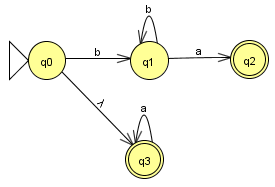
\includegraphics[width=0.5\textwidth]{img/q1/q1a.png}
                              \end{figure}

                        \item The language $\{w : w \text{ either has no consecutuve a's or no consecutive b's} \}$ with at most 5 states.

                              \textbf{Solution:}

                              \begin{figure}[h!]
                                    \centering
                                    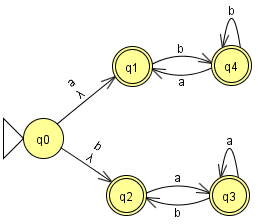
\includegraphics[width=0.5\textwidth]{img/q1/q1b.png}
                              \end{figure}

                              \newpage

                        \item The language $\{w : w \text{ contains an even number of a's or exactly two b's} \}$ with at most 6 states.

                              \textbf{Solution:}

                              \begin{figure}[h!]
                                    \centering
                                    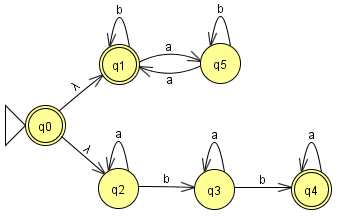
\includegraphics[width=0.5\textwidth]{img/q1/q1c.png}
                              \end{figure}

                        \item The language $\{ab,aab,aba \}^*$ with at most 4 states.

                              \textbf{Solution:}

                              \begin{figure}[h!]
                                    \centering
                                    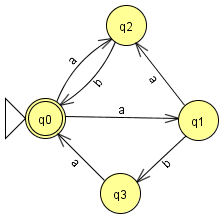
\includegraphics[width=0.4\textwidth]{img/q1/q1d.png}
                              \end{figure}

                  \end{enumerate}

                  \newpage
            \item[2.] [20 Points] Let $\Sigma = \{a,b \}$. Convert each NFA below to a DFA using the subset construction. Draw the transition diagram of your DFA, label the states of your DFA by subset of states of the original NFA.

                  \begin{enumerate}
                        \item[] a)
                              \begin{figure}[h!]
                                    \centering
                                    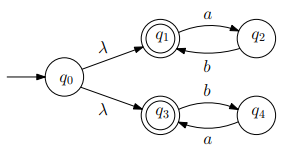
\includegraphics[width=0.6\textwidth]{img/q2/question2a.png}
                              \end{figure}

                              \textbf{Solution:} \textit{Note:} States with ``null'' in them represent the empty set ($\emptyset$).

                              \begin{figure}[h!]
                                    \centering
                                    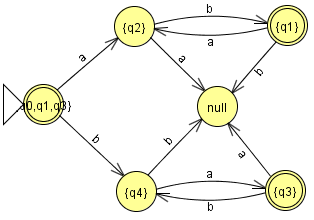
\includegraphics[width=0.6\textwidth]{img/q2/q2a.png}
                              \end{figure}

                              \newpage

                        \item[] b)
                              \begin{figure}[h!]
                                    \centering
                                    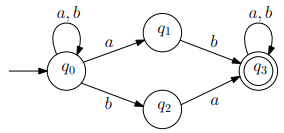
\includegraphics[width=0.6\textwidth]{img/q2/question2b.png}
                              \end{figure}

                              \textbf{Solution:}

                              \begin{figure}[h!]
                                    \centering
                                    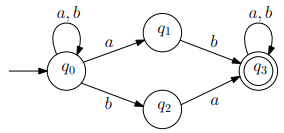
\includegraphics[width=0.6\textwidth]{img/q2/q2b.png}
                              \end{figure}
                  \end{enumerate}

                  \newpage
            \item[3.] [20 Points] Find a regular expression for each of the following languages.

                  \begin{enumerate}
                        \item $\{ba^nb^m : n \geq 3, m \geq 2 \}$

                              \textbf{Solution:} $$r = b(aaa)a^*(bb)b^*$$

                        \item
                              $
                                    \begin{aligned}[t]
                                          \{ w \in \{a,b \}^* : \text{every maximal } & \text{substring of } w \text{ consisting entirely of symbols $a$} \\ \text{is of length exactly 3} \}
                                    \end{aligned}
                              $

                              \textbf{Solution:} $$r = b^* + (b^*(aaa)b^*)^*$$

                        \item $\{w \in \{a,b \}^* : w \text{ does not contain $bab$ as a substring} \}$

                              \textbf{Solution:} $$r = a^*b^* + b^*a^* + (a^*b^*(aa)a^*b^*)^*$$

                        \item $\{w \in \{a,b\}^* : w \text{ begins with $bb$ and } n_b(w) \mod 3 = 0 \}$

                              \textbf{Solution:} $$r = (bba^*ba^*)^*$$
                  \end{enumerate}

      \end{enumerate}

\end{spacing}

\end{document}